\chapter*{Riassunto}
\chaptermark{Riassunto}
All'interno del Modello Standard, i neutrini sono descritti come particelle elusive, prive di massa e presenti in tre differenti sapori: elettronico, muonico e tauonico. Tuttavia, numerosi esperimenti degli ultimi decenni hanno confermato il fenomeno delle oscillazioni dei neutrini, processo possibile esclusivamente se queste particelle possiedono massa, che permette loro di trasformarsi da un sapore all'altro durante la propagazione. Le oscillazioni possono essere descritte attraverso una serie di parametri noti (come gli angoli di mixing e le differenze di massa al quadrato) ma le masse assolute dei neutrini e il loro ordinamento relativo (NMO) rimangono tutt'ora sconosciute. In questo contesto si colloca il rivelatore JUNO (Jiangmen Underground Neutrino Observatory), che rappresenta una delle migliori opportunità per fare luce su questo aspetto ancora irrisolto.

JUNO è un rivelatore multiobiettivo, situato in un laboratorio sotterraneo nel sud della Cina, con l'obiettivo principale determinare il NMO tramite la spettroscopia di antineutrini elettronici $\Bar{\nu}_e$ provenienti da due reattori nucleari situati a 52 km di distanza. Il nucleo dell'esperimento è costituito da $20\,\unit{kt}$ di scintillatore liquido (LS) contenuto nel Central Detector (CD), una sfera dal diametro di $35.4\,\unit{m}$ di materiale acrilico. Quest'ultima è inserita all'interno della Water Pool (WP), un cilindro che contiene $35\,\unit{kt}$ di acqua ultra pura. Entrambi i sotto-rivelatori sono composti da tubi fotomoltiplicatori in grado di osservare segnali di luce prodotti dalle particelle che attraversano JUNO. Grazie alle sue dimensioni e alla buona risoluzione energetica, JUNO dovrebbe permettere di determinare NMO con una significatività statistica di $3\sigma$ in sette anni di dati, oltre a contribuire allo studio di neutrini solari, atmosferici, da supernova e geoneutrini.

Uno degli aspetti cruciali per il successo dell’esperimento è la riduzione dei segnali di fondo, in particolare quello cosmogenico. Anche se JUNO è protetto da circa 700 m di roccia, un flusso residuo di muoni cosmici (stimato intorno a $\sim4\,\unit{mHz/m^2}$) può interagire con lo scintillatore liquido, producendo isotopi radioattivi che generano segnali all'interno del CD. Per questo motivo, è fondamentale sviluppare metodi efficaci per identificare e ricostruire la traccia dei muoni, così da poter applicare tecniche di veto.

Il lavoro presentato in questa tesi si concentra sull’analisi degli eventi candidati muoni dai primi dati raccolti da gennaio 2025 a marzo 2025, durante il riempimento del Central Detector con lo scintillatore. I muoni cosmici producono una quantità molto elevata di fotoni Cherenkov producono un gran numero di fotoni Cherenkov sia nel Central Detector che nella Water Pool, una segnatura che li rende individuabili indipendentemente dallo stato di riempimento con LS del rivelatore.

Per selezionare gli eventi candidati muoni sono stati utilizzati due approcci indipendenti. Il primo metodo si basa sulla \textbf{correlazione temporale} tra i trigger del Central Detector e quelli della Water Pool. Infatti, dato che il percorso dei muoni è rettilineo, i segnali dovuti al passaggio dei muoni registrati nella WP e nel CD si osservano a tempi consecutivi ravvicinati. Calibrando i parametri di selezione degli eventi in carica, questo metodo ha permesso di ottenere un rate di selezione di circa $4\,\unit{Hz}$.
Il secondo metodo, invece, si basa sul \textbf{clustering di carica} dei PMT della Water Pool. Questo approccio, integrato nel software ufficiale di JUNO, sfrutta la disposizione spaziale dei PMT per identificare "gruppi" di PMT attivati dai fotoni Cherenkov, caratteristica che indica il passaggio del muone. Tale tecnica risulta particolarmente efficace nel ricostruire l'intera traccia dell'evento candidato muone. Con questo metodo, il rate degli eventi candidati muoni è risultato leggermente superiore circa del $20\%$, confermando una discrepanza dovuta alla diversa natura della selezione: mentre il metodo di correlazione temporale osserva solo gli eventi che passano attraverso il CD, quello basato sul clustering include anche i muoni tangenti o appena esterni al Central Detector.

Il confronto tra i due metodi ha evidenziato che il metodo della correlazione temporale, pur risultando più stringente e riducendo il rischio di falsi positivi, fornisce informazioni limitate. Invece il metodo basato sul clustering di carica dei PMT della WP offre informazioni spaziali più dettagliate, come la posizione del centro del cluster, potendo in questo modo ricostruire la traccia del muone. L’analisi dell’angolo polare e azimutale della direzione ricostruita ha inoltre mostrato una buona compatibilità con le simulazioni Monte Carlo.

In conclusione, i due metodi proposti si sono dimostrati efficaci nella caratterizzazione del flusso di muoni in JUNO, in vista di una futura strategia di veto degli eventi cosmogenici derivati da muoni. Sebbene lo studio dei muoni sia ancora in fase di ottimizzazione e i due metodi rappresentino solo una parte della strategia complessiva di classificazione e caratterizzazione, un approccio combinato potrebbe rappresentare una soluzione promettente per migliorare la selezione e la ricostruzione degli eventi candidati muoni in JUNO.
\begin{figure}[ht]
    %Sub-percent precision measurement of neutrino oscillation parameters with JUNO
    \centering
    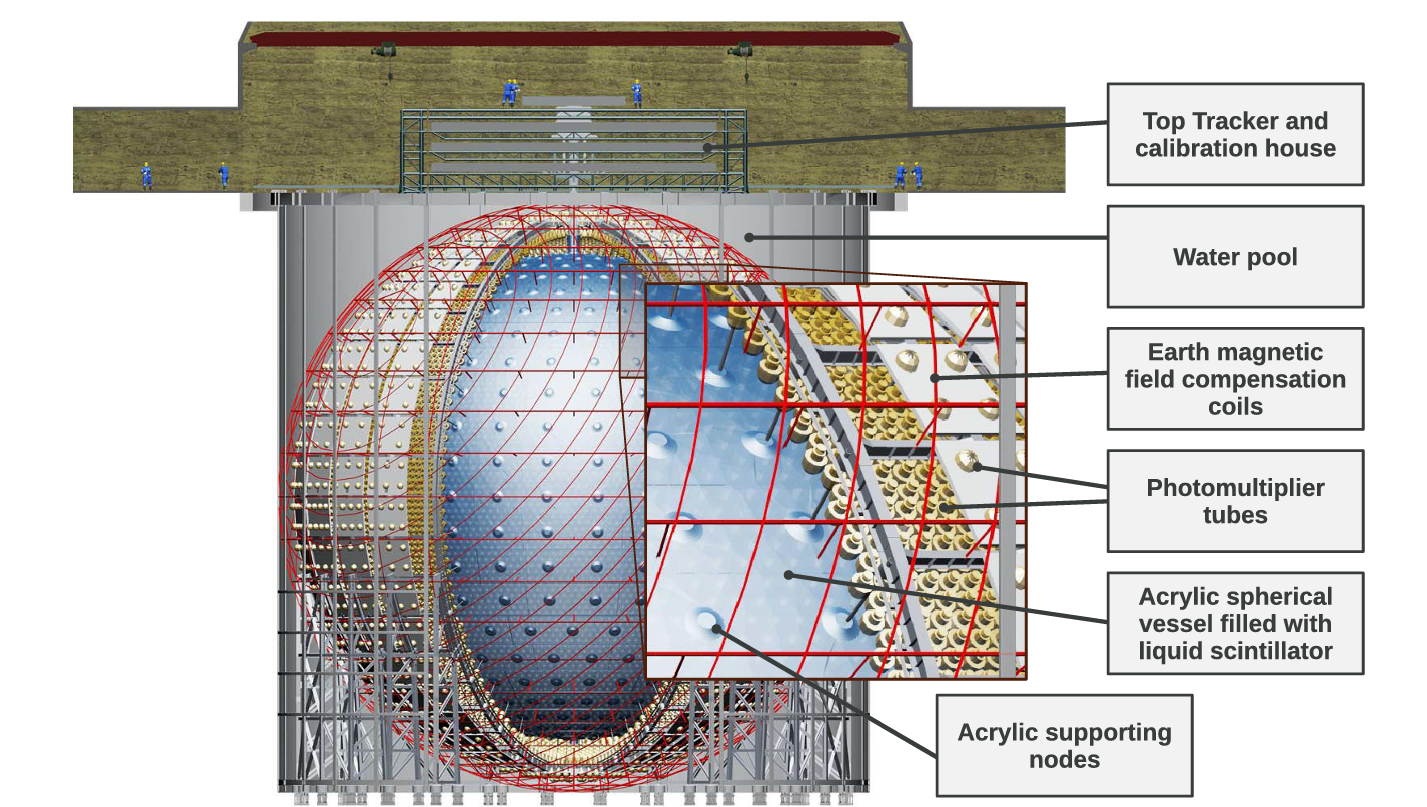
\includegraphics[width=1\textwidth]{Immagini/JUNO.png}
    \caption{Schema delle componenti principali di JUNO. Il diametro interno del Central Detector è di $35.4\,\unit{m}$ mentre il diametro della struttura in acciaio inossidabile in cui sono posizionati i PMT della Water Pool è di $40.1\,\unit{m}$ \cite{JUNO:2022mxj}.}
    \label{Fig:JUNO}
\end{figure}